\section{Introducción}
En este laboratorio se realizó un programa que simula el comportamiento del código genético, es decir, la traducción de una secuencia de nucleótidos en el ARN, a una secuencia de aminoácidos, tal y como sucede en los seres vivos. La secuencia de ARN es caracterizada por cuatro bases nitrogenadas, representadas con las letras A, G, C y U (adenina, guanina, citosina y uracilo, respectivamente). Estos nucleótidos se agrupan de 3 en 3, grupos que se denominan codones, y cada codón se traduce en un aminoácido. Existen 3 codones especiales que no se traducen en aminoácidos, sino que marcan el inicio y final de una cadena.

El funcionamiento del presente programa se basa en un archivo de origen (\texttt{.txt}) en el cual se encuentran las cadenas de nucleótidos, una serie de métodos que se encargan de la traducción y, finalmente, la escritura de la cadena de aminoácidos resultante en un archivo de destino. Se crea una clase llamada FILEUTIL que, haciendo uso de la librería \texttt{fstream} de C++, se encarga de las operaciones de apertura, lectura y escritura de los archivos; y una clase TRANSLATOR que lleva a cabo todo el proceso de traducción.


\subsection{Objetivos}
\begin{enumerate}
\item Familiarizarse con el lenguaje de programación C++ y el paradigma de orientación a objetos.
\item Resolver un problema mediante el uso de arreglos, funciones, clases y memoria dinámica.
\item Practicar el uso de makefiles, la documentación con Doxygen y el control de versiones en GitLab.
\item Utilizar las herramientas de manejo de archivos de C++.
\end{enumerate}

\section{Enunciado}
Escriba y documente (con Doxygen) un programa en C++, usando orientación a objetos, que genere los aminoácidos a partir de los codones de un código genético (ARN) cualquiera. Para esto,
el programa recibe de la línea de comandos dos rutas, el archivo de entrada y el archivo de salida.\\
El archivo de entrada estará compuesto por una serie de bases nitrogenadas (A, G, C, U) múltiplo de 3, que siempre empieza y termina por un codón de parada.\\
Archivo de entrada con múltiples línea de datos.\\
En archivo de salida estarán los aminoácidos que se traducen a partir de las bases nitrogenadas.
Use la figura \ref{fig:1} o \url{https://en.wikipedia.org/wiki/Genetic_code#RNA_codon_table}.

\begin{figure}[H]
\centering
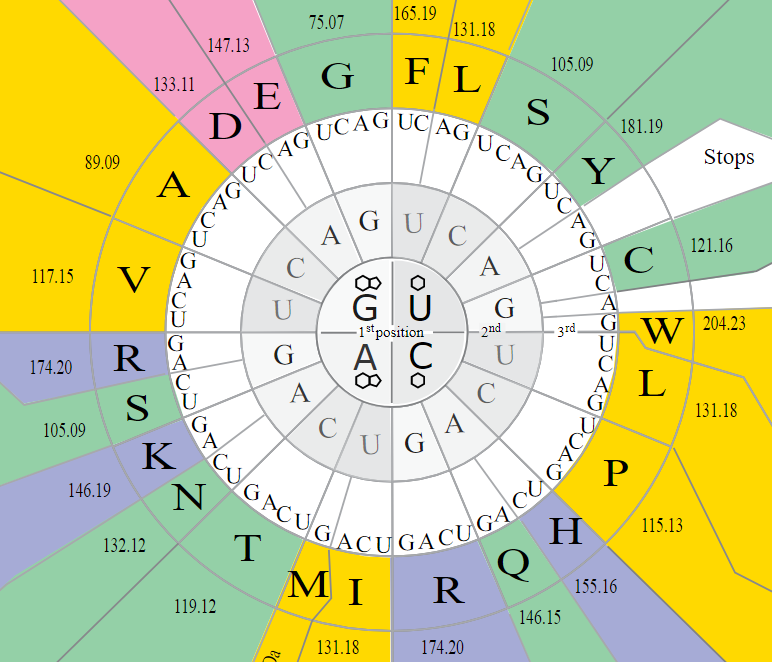
\includegraphics[width=0.6\textwidth]{imgs/Labo2/cod-gen}
\caption{Tabla de conversión ARN a aminoácido}
\label{fig:1}
\end{figure}

\subsection{Ejemplo 1}
El siguiente archivo de entrada:
\begin{lstlisting}[backgroundcolor=\color{verdito}]
UAACCUUCUACUACGUAG
\end{lstlisting}
Produce el siguiente archivo de salida:
\begin{lstlisting}[backgroundcolor=\color{verdito}]
PSTT
\end{lstlisting}

\subsection{Ejemplo 2}
El siguiente archivo de entrada:
\begin{lstlisting}[backgroundcolor=\color{verdito}]
UAACCUUCUACUACGUAG
UAGUCUCCUACGACUUUA
UAACCUUCUACUACGUAG
UAGUCUCCUACGACUUUA
\end{lstlisting}
Produce el siguiente archivo de salida:
\begin{lstlisting}[backgroundcolor=\color{verdito}]
TTPS
SPTT
TTPS
SPTT
\end{lstlisting}

\subsection{Detalles}
Cree al menos dos clases \texttt{Translator} y \texttt{FileUtil}. Los métodos mínimos para ambas clases se muestran en las tablas \ref{T1} y \ref{T2}. Además desarrolle la función \texttt{main} en un archivo aparte.


\begin{table}[H]
\begin{center}
    \begin{tabular}{ |c|c|c|c| }
    	\hline
    	\cellcolor{cl} \textbf{Tipo de retorno} & \cellcolor{cl} \textbf{Nombre del método} & \cellcolor{cl} \textbf{Argumentos} & \cellcolor{cl} \textbf{Detalle}\\ \hline \hline
         & Translator &   & Método constructor\\  \hline
         & $\sim$Translator & & Método destructor\\ \hline
         string & translate & string s & Método que traduce 1 string s\\ & & & en otro string usando las\\ & & & reglas del código genético\\ \hline
         string* & translate & string* s, int n & Método que traduce n strings\\ & & & s en otros usando las reglas\\ & & &  del código genético\\ \hline
    \end{tabular}
\end{center}
\label{T1}
\caption{Métodos de la clase \texttt{Translator}}
\end{table}


\begin{table}[H]
\begin{center}
    \begin{tabular}{ |>{\centering\arraybackslash}m{3.5cm}|>{\centering\arraybackslash}m{3.9cm}|>{\centering\arraybackslash}m{3cm}|>{\centering\arraybackslash}m{5cm}| }
    	\hline
    	\cellcolor{cl} \textbf{Tipo de retorno} & \cellcolor{cl} \textbf{Nombre del método} & \cellcolor{cl} \textbf{Argumentos} & \cellcolor{cl} \textbf{Detalle}\\ \hline \hline
         & FileUtil & string s, io\_base::openmode p & Método constructor, usa el archivo indicado por la ruta s\\ \hline
         & $\sim$FileUtil  & & Método destructor\\ \hline
         string & read & & Método que lee una línea del
\\ & & & archivo asociado al objeto\\ \hline
         string* & readLines & & Método que lee todas las líneas\\ & & & del archivo asociado al objeto\\ \hline
         int & write & string s & Método que escribe una línea
\\ & & & al archivo asociado al objeto\\ \hline
         int & write & string* s, int n & Método que escribe n líneas\\ & & & al archivo asociado al objeto\\ \hline
    \end{tabular}
\end{center}
\label{T2}
\caption{Métodos de la clase \texttt{FileUtil}}
\end{table}

Haga una corrida de prueba y genere archivos de ejemplo con entradas predefinidas para verificar la efectividad de su código.

\begin{itemize}
\item Recuerde que la idea de este laboratorio es familiarizarse con el uso de memoria dinámica, arreglos, funciones, orientación a objetos y en general la sintaxis de C++.
\item Recuerde también que por cada \texttt{new} que utilice, necesita un \texttt{delete}, sino tendrá fugas de memoria.
\item El código genético empezará y finalizará SIEMPRE con un codón de parada
\end{itemize}

\newpage

%%%%%%%%%%%%%%%%%%%%%%%%%%%%%%%%%%%%%%%%%%%%%%%%%%%%%%%%%%%%%%%%%%%%
\section{Solución}
%%%%%%%%%%%%%%%%%%%%%%%%%%%%%%%%%%%%%%%%%%%%%%%%%%%%%%%%%%%%%%%%%%%%

\subsection{Clase \texttt{FileUtil}}
Esta es la clase que se encarga del manejo de archivos; en este caso, apertura, cierre, lectura y escritura. El archivo header (\texttt{FileUtil.h}) contiene las definiciones de los métodos y atributos. En la sección pública se colocan las definiciones de los métodos constructor, destructor, los de lectura y escritura, y dos métodos auxiliares para determinar la cantidad de líneas del archivo. En la parte privada, se declaran los atributos.


\begin{minted}[linenos,autogobble,bgcolor=bg,breaklines,fontsize=\footnotesize ]{c++}
#include <string>
#include <iostream>
using namespace std;

class FileUtil
{
  public:
  	FileUtil(string s, ios_base::openmode p);
  	~FileUtil();
  	string read();
  	string* readLines();
  	int write(string s);
  	int write(string* s, int n);
    void countNumberLines();
    int getNumberLines();
  private:
    //Numero de lineas.
    int numLines;
    //Dirección de lectura.
    string ruta;
    //Modo de lectura.
  	ios_base::openmode modo;
    //Linea leida.
    string line;
    //Puntero con la direccion del arreglo de las lineas leidas.
    string* lines;

};
\end{minted}

\subsubsection{Implementación}

\begin{itemize}
\item \textbf{Método constructor:}\\
El método constructor recibe dos argumentos, que corresponden a la ruta del archivo a procesar, y el modo de procesamiento. Este modo es una variable del tipo \texttt{ios\_base::openmode}, y en este caso existen dos posibles modos válidos: \texttt{in} y \texttt{out}. Estos argumentos se asignan a los atributos ``ruta'' y ``modo'', respectivamente. Además en el constructor se inicializan los atributos ``lines'' y ``numLines''.


\begin{minted}[linenos,autogobble,bgcolor=bg,breaklines,fontsize=\footnotesize ]{c++}
FileUtil::FileUtil (string s, ios_base::openmode p)
{
  this->ruta = s;
  this->modo = p;
  this->numLines = 0;
  int n = FileUtil::getNumberLines();
  this->lines = new string[n];
}

};
\end{minted}

\item \textbf{Método destructor:}\\
En el método destructor se hace la liberación de memoria correspondiente al atributo de tipo arreglo de tamaño variable, ``lines''.
\begin{minted}[linenos,autogobble,bgcolor=bg,breaklines,fontsize=\footnotesize ]{c++}
FileUtil::~FileUtil()
{
  delete [] this->lines;
}
\end{minted}


\item \textbf{Método \texttt{read()}:}\\

Este método usa la biblioteca \texttt{fstream} para crear un objeto llamado ``myFile'', sobre el cual se ejecutan las operaciones. En este caso, se lee una única línea, y el contenido de ésta se asigna al atributo ``line'', de tipo string, que es el valor de retorno y que luego se pasará a los métodos de traducción. En este caso, se asigna directamente el valor a ``numLines'' = 1. 

\begin{minted}[linenos,autogobble,bgcolor=bg,breaklines,fontsize=\footnotesize ]{c++}
string FileUtil::read(){
  fstream myFile(this->ruta.c_str(),this->modo);
  if (myFile.is_open())
 {
    getline(myFile,this->line);
    this->numLines = 1;
    myFile.close();
  }
  return this->line;
}
\end{minted}

\item \textbf{Método \texttt{readLines()}:}\\

Este método permite leer un archivo que posee múltiples líneas de texto. Se usa una variable auxiliar ``count'' para recorrer las líneas. En cada línea leída, su contenido se asigna al atributo ``line'', y éste se agrega al arreglo de strings llamado ``lines[]'', que es el retorno de la función. De esta manera, se tiene que este método retorna un arreglo de strings que contiene todas las líneas de texto leídas del archivo de origen. 

\begin{minted}[linenos,autogobble,bgcolor=bg,breaklines,fontsize=\footnotesize ]{c++}
string* FileUtil::readLines(){
  int count = 0;
  fstream myFile(this->ruta.c_str(),this->modo);
  if (myFile.is_open())
 {
    while (getline(myFile,this->line))
    {
      this->lines[count] = this->line;
      //cout << this->line << '\n';
      count++;
    }
    myFile.close();
  }
  return this->lines;
}
\end{minted}


\item \textbf{Métodos \texttt{write()}:}

El primer método \texttt{write()} se encarga de escribir una única línea de texto en un archivo. Su argumento es un string que contiene el texto a escribir. En este caso, el valor de retorno es 0 si el proceso se llevó a cabo exitosamente, y 1 si ocurrió algún error. 

\begin{minted}[linenos,autogobble,bgcolor=bg,breaklines,fontsize=\footnotesize ]{c++}
int FileUtil::write (string s)
{
  fstream myFile(this->ruta.c_str(),this->modo);

  if (myFile.is_open())
  {
    myFile << s;
    myFile.close();
    return 0;
  }
  else
  {
    cout << "Unable to open file";
    return 1;
  }
}
\end{minted}

El segundo método llamado \texttt{write()}, recibe como argumento un arreglo de strings \texttt{s} con el texto a escribir en un archivo, y un entero \texttt{n} que indica el total de líneas que se desea escribir. Se usa un incrementador llamado ``count'' que sirve para recorrer el arreglo y accesar su contenido, asignándoselo al stream ``myFile''.

\begin{minted}[linenos,autogobble,bgcolor=bg,breaklines,fontsize=\footnotesize ]{c++}
int FileUtil::write (string* s, int n)
{
  fstream myFile(this->ruta.c_str(),this->modo);
  if (myFile.is_open())
  {
    for (int count = 0; count < n; count++)
    {
      myFile << *(s+count);
      myFile << endl;
    }
    myFile.close();
    return 0;
  }
  else
  {
    cout << "Unable to open file";
    return 1;
  }
}
\end{minted}


\item \textbf{Métodos auxiliares:}

El método \texttt{getNumberLines()} devuelve el número de líneas de texto de un archivo. Para esto, llama al método \texttt{countNumberLines()}, el cual recorre todas las líneas del archivo, incrementando un contador llamado ``numLines'' (que es un atributo de esta clase). El valor final de numLines es el retorno de este método.

\begin{minted}[linenos,autogobble,bgcolor=bg,breaklines,fontsize=\footnotesize ]{c++}
int FileUtil::getNumberLines()
{
  FileUtil::countNumberLines();
  return this->numLines;
}
\end{minted}


\begin{minted}[linenos,autogobble,bgcolor=bg,breaklines,fontsize=\footnotesize ]{c++}
void FileUtil::countNumberLines()
{
  this->numLines = 0;
  fstream myFile(this->ruta.c_str(),this->modo);
  if (myFile.is_open())
 {
    while (getline(myFile,this->line))
    {
      this->numLines++;
    }
    myFile.close();
  }
}

\end{minted}

\end{itemize}
\subsection{Clase \texttt{Translator}}

Esta clase es la que contiene los métodos encargados de la traducción de los codones. En el header (\texttt{Translator.h}) se definen los métodos y atributos.
\begin{minted}[linenos,breaklines,bgcolor=bg,fontsize=\footnotesize ]{c++}
#include <string>
#include <iostream>
using namespace std;

class Translator {
	public:
    	Translator();
    	~Translator();
    	string translate (string s);
    	string* translate (string* s, int n);
    	string asociar(int i, int j);
    	string error();
    private:
};
\end{minted}

\subsubsection{Implementación}

\begin{itemize}

\item \textbf{Método \texttt{translate(string s)}:}

Es el método principal de la clase (y de todo el programa), ya que es el que realiza toda la comparación necesaria para la traducción. Se le pasa como argumento un string que corresponde a una línea de texto, previamente obtenida de un archivo \texttt{.txt}.

Las primeras operaciones que se realizan son de conteo de cantidad de caracteres y cantidad de tríos de letras (codones) en la línea de texto.

\begin{minted}[linenos,breaklines,bgcolor=bg,fontsize=\footnotesize ]{c++}
string Translator::translate (string s) {
  string codones = s; // Codones leidos de una fila del archivo .txt
  int tamano = codones.size(); // Cantidad de letras en la fila  
  int cantidadTrios = tamano / 3; // Cantidad de grupos de tres letras
\end{minted}
Se crea el arreglo llamado ``arregloTrios'', en el cual, cada elemento será un codón. Como este arreglo es de tamaño variable, se utiliza memoria dinámica.

\begin{minted}[linenos,breaklines,bgcolor=bg,fontsize=\footnotesize ]{c++}
  string* arregloTrios;
  arregloTrios = new string[cantidadTrios];
\end{minted}

Igualmente se crea el arreglo ``traducido'', el cual va a contener las letras correspondientes a los aminoácidos, una vez terminada la traducción.

\begin{minted}[linenos,breaklines,bgcolor=bg,fontsize=\footnotesize ]{c++}
  string* traducido;
  traducido = new string[cantidadTrios-2];
\end{minted}

Posteriormente, se incluyen las rutinas de verificación de condiciones necesarias. La primera, es que la cantidad de letras en el string de origen sea múltiplo de 3; para esto, se incluye todo el código posterior dentro de un \texttt{if}. 

\begin{minted}[linenos,breaklines,bgcolor=bg,fontsize=\footnotesize ]{c++}
	if (tamano % 3 == 0 ){ 
		...
	} else {
		error();
		cout << "Error: cantidad de caracteres no es multiplo de 3." << endl;
  	}
\end{minted}

El siguiente bloque asigna a cada elemento de arregloTrios un conjunto de 3 letras del string original:

\begin{minted}[linenos,breaklines,bgcolor=bg,fontsize=\footnotesize ]{c++}
	int i = 0;
	int c = 0;
	for (int x = 0; x < cantidadTrios; x++ ){
		arregloTrios[i] = codones.substr(c, 3); // La funcion substr(a,b) guarda b letras de la string desde la posicion a
		i++;
		c += 3;
   		 }
\end{minted}

Luego, habiendo definido previamente los codones de parada válidos:

\begin{minted}[linenos,breaklines,bgcolor=bg,fontsize=\footnotesize ]{c++}
  string cdnparada1 = "UGA";
  string cdnparada2 = "UAG";
  string cdnparada3 = "UAA";
\end{minted}

Se procede a verificar que la línea de texto evaluada comience y termine con un codón de parada válido:

\begin{minted}[linenos,breaklines,bgcolor=bg,fontsize=\footnotesize ]{c++}
    if ( !(arregloTrios[0] == cdnparada1 || arregloTrios[0] == cdnparada2 || arregloTrios[0] == cdnparada3 ) ){ //Compara el trio del inicio
		error();
    cout << "Error: la hilera no tiene codones de parada validos." << endl;
		
	} else if (!(arregloTrios[cantidadTrios-1] == cdnparada1 || arregloTrios[cantidadTrios-1] == cdnparada2 || arregloTrios[cantidadTrios-1] == cdnparada3)){ //Compara el trio del final
		error();
    cout << "Error: la hilera no tiene codones de parada validos." << endl;
		
	} else { //trios de parada existen
		cout << "La hilera tiene codones de parada validos." << endl;
\end{minted}
La siguiente condición consiste en verificar que todos los caracteres contenidos en el texto sean válidos, es decir, ``A'', ``U'', ``G'' o ``C''.

\begin{minted}[linenos,breaklines,bgcolor=bg,fontsize=\footnotesize ]{c++}
		for (int d = 0; d < tamano; d++){
			letras [d] = codones.substr(d,1); //guarda las letras una por una como string
		}

		for (int t=0;t<tamano;t++){
  		// cout << letras[t] <<endl;
  		if (letras[t] == "A" || letras[t] == "C" || letras[t] == "G" || letras[t] == "U"  ) {
  			cout << letras [t] << ": Todo bien, letra valida." << endl;
  			} else {
  			error();
        cout << letras[t] << ": Error: letra no valida." << endl;
  			}
  		}  
\end{minted}

Habiéndose cumplido todas las condiciones, se procede luego con la traducción. En esta sección se empieza creando un \texttt{string} en donde se va a almacenar las letras de la traducción. Con un \texttt{for()} que ignora los tríos del principio y el final (ya se verificó que son codones de parada válidos, por lo que no se traducen) se compara cada codón del string que se quiere traducir \texttt{arregloTrios[]} con los codones de que conforman las posibles combinaciones de letras de las bases nitrogenadas. Cuando uno de estos tríos coincida se llama al método \texttt{asociar()} al que se le envían como argumentos la posición del codón que coincidió para que así asocie a cuál aminoácido corresponde. Lo que retorna la función \texttt{asociar()} se almacena en el \texttt{string} creado anteriormente, al que se le van agregando los resultados utilizando la función \texttt{append()} de las bibliotecas de C++.

\begin{minted}[linenos,breaklines,bgcolor=bg,fontsize=\footnotesize ]{c++}
string traducido;
  	for (int r = 1; r < cantidadTrios-1; r++ ){ //Ignorando el primer y ultimo trios porque ya se comprobó que son de parada
  		for (int p = 0; p < 64; p++){
  			if ( arregloTrios[r] == cdntraduccion[p] ) {
  				string letra = asociar(p, r-1);
  				traducido.append(letra);
  			}
  		}
  	}
\end{minted}


\item \textbf{Método \texttt{translate(string* s, int n)}:}

Es el método encargado de la traducción de un archivo con varias líneas de codones. Recibe como argumento un puntero \texttt{string *s} con dirección del primer elemento de un arreglo de \texttt{string}s donde se guardan las cadenas que se van a traducir. También se le envía un entero \texttt{n} que le indica al método la cantidad de elementos que posee el arreglo, es decir, la cantidad de líneas que se quieren traducir.

\begin{minted}[linenos,breaklines,bgcolor=bg,fontsize=\footnotesize ]{c++}
string* Translator::translate (string* s, int n){
  string* traduccion = new string [n];
\end{minted}
Cuando se obtienen los parámetros se reserva memoria dinámica (utilizando \texttt{new}) para un nuevo puntero que almacena la dirección de la traducción realizada,este puntero tiene una dimensión \texttt{n}, como se observa en la línea 2.

\begin{minted}[linenos,breaklines,bgcolor=bg,fontsize=\footnotesize ]{c++}
  for (int q = 0; q < n; q++ ){
    traduccion[q] = translate(s[q]);
  }
\end{minted}
Luego se procede a llamar al método \texttt{translate()} varias veces mediante un ciclo \texttt{for()}, \texttt{n} veces. En donde se le envían cada una de las líneas que se quieren traducir, y lo que retorna este método se almacena en la variable creada anteriormente.

\begin{minted}[linenos,breaklines,bgcolor=bg,fontsize=\footnotesize ]{c++}
  return traduccion;
\end{minted}

Finalmente se procede a devolver el puntero que apunta al arreglo que almacena las traducciones.

\item \textbf{Método \texttt{asociar()}:}

Método auxiliar utilizado para asociar directamente un codón (un elemento del arreglo arregloTrios[ ] con su correspondiente letra (aminoácido). Recibe la posición con la que coincidió el trío de codones, y la compara mediante un \texttt{switch()} para saber a cuál aminoácido corresponde. Cada uno de los 64 casos corresponde a un aminoácido representado por la una única letra. La función regresa esta letra en forma de \texttt{string}.

\begin{minted}[linenos,breaklines,bgcolor=bg,fontsize=\footnotesize ]{c++}
string Translator::asociar (int i, int j){
    string letra;
    switch(i){
      case 0:
        letra = "G";
  		break;
      case 1:
        letra = "G";
  		break;
      ...
      ...
      ...
      case 63:
        letra = "F";
  		break;
      }
    return letra;
}
\end{minted}


\item \textbf{Método \texttt{error()}:}

Se incluyó un método para mostrar un mensaje de error cuando se presente alguna situación indeseada en la ejecución del programa.

\begin{minted}[linenos,breaklines,bgcolor=bg,fontsize=\footnotesize ]{c++}
void Translator::error(){
  cout << "|||||||| ERROR EN LA EJECUCION DEL PROGRAMA ||||||||" << endl;
}
\end{minted}
\end{itemize}


\section{Resultados}

Una vez que se tienen todos los códigos listos y en sus respectivas carpetas, se compila con un \texttt{makefile} y se ejecuta. El programa solicita mediante la terminal que se ingrese la ruta donde se ubica el archivo \texttt{.txt} con las cadenas a traducir, y posteriormente nos solicita la ruta del archivo en donde se va a escribir la traducción. Si no se encuentra ningún problema, se crea correctamente el archivo de salida. Este archivo se puede leer con cualquier editor de texto, en la Figura \ref{fig:trans1} se muestra a la izquierda el archivo que contiene la cadena a traducir. Y a la derecha se puede observar el archivo en donde se escribió la traducción del mismo. En este caso corresponde a únicamente una línea de 4 letras. 

\begin{figure}[htbp]
\centering
\subfigure[Cadena de codones.]{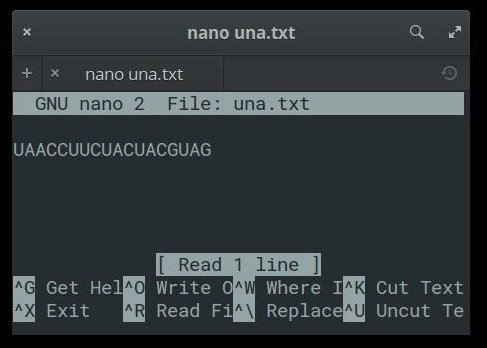
\includegraphics[width=54mm]{imgs/Labo2/INuna.jpeg}}
\subfigure[Traducción de la cadena.]{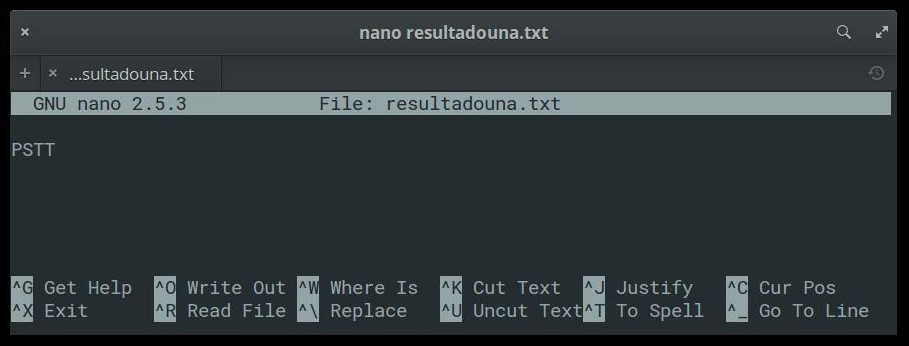
\includegraphics[width=101.5mm]{imgs/Labo2/OUTuna.jpeg}}
\caption{Traducción de una única línea.} \label{fig:trans1}
\end{figure}

Cuando al programa se le indica una ruta de un archivo con varias líneas como el que se observa en la imagen izquierda de la Figura \ref{fig:trans2}, este se ejecuta de igual manera, y escribe un archivo con la traducción correspondiente como se observa en la imagen de la derecha.

\begin{figure}[htbp]
\centering
\subfigure[Varias cadenas de codones.]{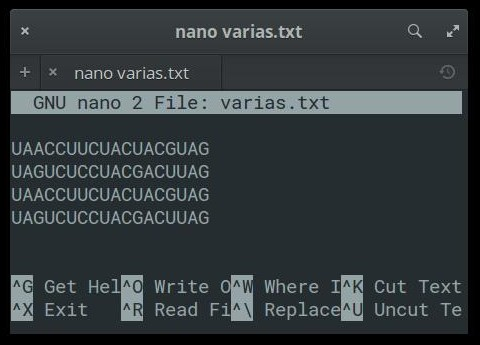
\includegraphics[width=54mm]{imgs/Labo2/INvarias.jpeg}}
\subfigure[Traducción de las cadenas.]{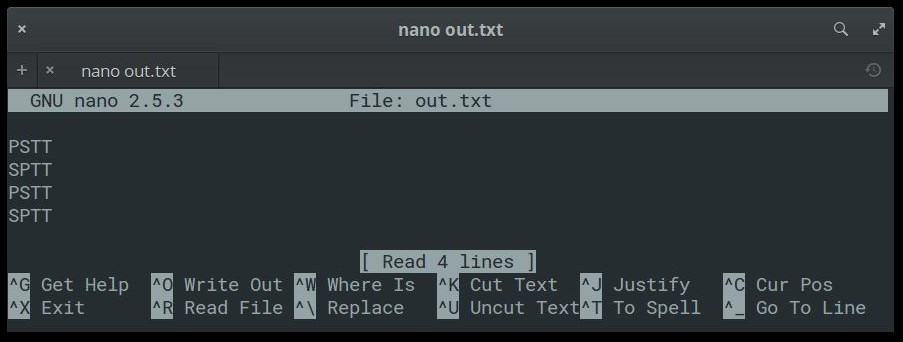
\includegraphics[width=102mm]{imgs/Labo2/OUTvarias.jpeg}}
\caption{Traducción de varias cadenas de codones.} \label{fig:trans2}
\end{figure}

\section{Conclusiones}
El objetivo principal del laboratorio se cumplió satisfactoriamente. Se logró familiarizarse con los comandos de C++ y el paradigma de programación orientada a objetos. También es importante notar el uso del concepto de reserva de memoria dinámica, así como su debida liberación después de su uso. Además se practicó la correcta documentación del código utilizando \texttt{Doxygen}, y la compilación mediante un \texttt{makefile}. 
